\chapter{State of the Art}


\section{Nicht Physikalisch basierte Methoden}

Wie schon bereits erwähnt wird in den nicht physikalisch basierten Methoden meist auf das Voronoi Diagramm zurückgegriffen. 

Ausgehend von einer endlichen Menge an verschiedenen, isolierten Punkten in einem Raum, werden alle Orte mit dem nächstgelegenen Punkt der Punktmenge assoziiert.
Das Ergebnis ist eine Unterteilung des Raumes in eine Menge von Regionen, die sogenannten Voronoi Zellen, die zusammen das Voronoi Diagramm bilden, 
wie in Abbildung \ref{fig:voronoi1} zu sehen ist \cite{Okabe.SpatialTessellationsVoronoi}.


\begin{figure}[H]
    \centering
    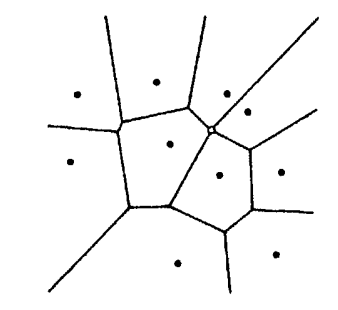
\includegraphics[width=0.35\linewidth]{PICs/basicVoronoi.PNG}
    \caption{Voronoi Diagramm \protect\cite{Okabe.SpatialTessellationsVoronoi}}
    \label{fig:voronoi1}
\end{figure}

Diese Voronoi Zellen werden als Primitive genutzt, um zerstörbare 3D Regionen zu repräsentieren, können schnell und einfach berechnet werden und auf praktisch alle 3D-Modelle
angewendet werden \cite{Najim.DynamicFracturing}.

Um nun Risse, Brüche oder Fragmente zu erzeugen wird ein Voronoi Diagramm konstruiert, indem im Innenraum und an den Kanten jedes Polygons zusätzliche Punkte erzeugt werden. 
Anschließend wird die resultierende Punktemenge trianguliert, inklusive der Kanten des Polygons, und infolgedessen das Voronoi Diagramm gebildet. 
Zum Schluss werden jene Kanten des Voronoi Netzes ausgeschnitten, welche über das Polygon hinausgehen. Das Ergebnis ist eine Sammlung von kleineren Polygonen, die zusammen
das ursprüngliche Polygon ergeben \cite{Raghavachary.FractureGenerationOnPolygonalMeshes}.

\begin{figure}[H]
    \centering
    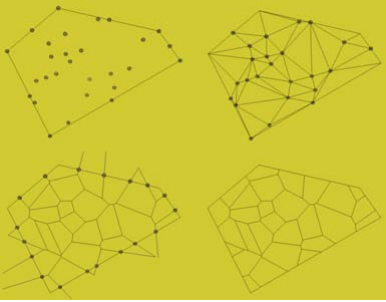
\includegraphics[width=0.5\linewidth]{PICs/voronoiSteps.PNG}
    \caption{Erstellung eines Voronoi Netzwerkes eines Polygons \protect\cite{Raghavachary.FractureGenerationOnPolygonalMeshes}}
    \label{fig:voronoi2}
\end{figure}

In Abbildung \ref{fig:voronoi2} werden die oben genannten Schritte grafisch dargestellt.

Um nun Verfeinerungen bei der Fragmentierung des Polygons an bestimmten Stellen vorzunehmen, muss nur die Punktmenge an eben diesen Stellen erhöht werden. Dadurch ergeben
sich bei der Erstellung des Voronoi Diagramms kleinere Polygone. Dies ist nützlich um beispielsweise den Eintreffpunkt eines Projektiles, oder 
den Auftreffpunkt eines herunterfalllenden Gegenstandes genau zu definieren. 




genralized in a variety of ways (chapter 3 in okabe)
data structures to represent voronoi (chapter 4)


\section{Physikalisch basierte Methoden}

\subsection{Mass-Spring Model}

Diese Technik basiert darauf, dass bestimmte Punkte eines 3D-Objektes mit Federn miteinander verbunden sind und entfernt werden, wenn diese einer bestimmten Belastung
ausgesetzt sind. Diese Belastung basiert auf einer bestimmten Schwelle die abhängig ist von der Länge der Feder und des Materials des 3D-Objektes. 

\subsection{Finite element methods}

